\documentclass[a4paper, 10pt]{article}

\usepackage{amsmath}
\usepackage{siunitx}
\usepackage{graphicx}
\usepackage[T1]{fontenc}
\usepackage[utf8]{inputenc}
\usepackage[english]{babel}
\usepackage[sc]{mathpazo}
\usepackage{color}

% Various spacing parameters
\usepackage{microtype}
\usepackage[margin=3.5cm]{geometry}
\linespread{1}
\parindent 0pt
\parskip 4pt

% Helping functions
\newcommand{\pdiff}[2]{\frac{\partial #1}{\partial #2}} % Partial derivative

% Spacing inside description environment
\usepackage{enumitem}
\setlist[description]{style=multiline,leftmargin=.8cm,parsep=4pt}

\title{Fluid Dynamics + Turbulence (fall 2018)\\Homework Problems III + voluntary Exercises}
\author{}
\date{}

%----------------------------------------------------------------------------------------

\begin{document}
\maketitle

\large{
\textbf{Posted:}

\today

\bigskip
\textbf{Deadline for submission of homework problem:}

September 25 (Tuesday) at 08:30 am (on Blackboard).
}

\bigskip

\section*{Homework problem 3.1: Mass flux and pressure in a 2-dimensional flow}
Consider the following 2D flow field:
\begin{equation}
\vec{u}(x,y)=-ax\vec{e}_x+ay\vec{e}_y
\end{equation}
for $x\geq0$ and $a$ some positive constant. It could be the flow field of an inviscid fluid approaching a wall at $x=0$ from the right. \newline

{\bf (a)} Determine the streamfunction $\Psi(x,y)$.\newline

{\bf (b)} Sketch the flow field. In particular mark the stagnation point at (0,0) and draw the streamlines connected to it. \newline

{\bf (c)} Show that the flow is incompressible and irrotational. \newline

{\bf (d)} Show that the mass flux
\begin{equation}
\rho\int_{y_1}^{y_2} u_xdy=\rho(\Psi(x,y_2)-\Psi(x,y_1))
\end{equation}
between the two points $(x,y_1)$ and $(x,y_2)$ can be expressed as the difference between the values of two streamlines. Calculate the mass flux between the two points $P_1=(10,0)$ and $P_2=(10,1)$. Is it bigger or smaller compared to the mass flux between $P_3=(1,0)$ and $P_4=(1,10)$? \newline

{\bf (e)} Assume that the fluid is inviscid and use the Bernoulli equation along the wall streamlines to find the pressure distribution at the wall:
\begin{equation}
p(x=0,y) = p_\mathrm{stagnation}-\frac{1}{2}\rho a^2y^2,
\end{equation}
where $p_\mathrm{stagnation} = p(0,0)$ is the (unknown) pressure at the stagnation point and $\rho$ is the density of the fluid. \newline

{\bf (f)} Put $\vec{u}$ into the Navier-Stokes equation. Do not assume the fluid to be inviscid, but show anyhow that the result above generalizes to $x>0$:
\begin{equation}
p(x,y) = p_\mathrm{stagnation}-\frac{1}{2}\rho a^2 (x^2+y^2)
\end{equation}
and sketch this pressure distribution.

\section*{Homework problem 3.2: Potential flow}
What potential flow is described by the following velocity potential?
\begin{equation}
\Phi(x,y) = \frac{m}{2\pi}\ln\sqrt{(x-a)^2 + y^2} + \frac{m}{2\pi}\ln\sqrt{(x+a)^2+y^2}
\end{equation}

\begin{description}
	\item[(a)]
	Determine the velocity components $v_x$ and $v_y$.
	\item[(b)]
	Determine the stream function $\Psi(x,y)$.
	
	\textit{Hint, you may need the following equations to determine the stream function.}
	\begin{equation*}
	\int\frac{1}{1+x^2}dx=\arctan x
	\end{equation*}
	\begin{equation*}
	\arctan \frac{1}{x} = -\arctan x\pm\frac{\pi}{2}
	\end{equation*}
	\item[(c)]
	Visualize the streamlines by plotting the contour lines of the stream function.
	\item[(d)]
	Why does the line $x=0$ represent a streamline? Determine the velocity components $v_x$ and $v_y$ at $x=0$.
\end{description}



\newpage


\section*{Exercise 3.1}
Show that for a potential flow the streamlines and the isopotential lines are orthogonal to each other. The streamlines are characterized by the stream function $\Psi(x,y)=\mathrm{constant}=c_1$, and the isopotential lines are characterized by the velocity potential $\Phi(x,y)=\mathrm{constant}=c_2$.

\section*{Exercise 3.2}
The velocity potential
\begin{equation}
\Phi(x,y) = \frac{m}{2\pi}\ln\sqrt{x^2+y^2}=\frac{m}{2\pi}\ln r
\end{equation}
describes the potential flow resulting from an ideal source located at the origin; see the figure below.

\begin{figure}[h!]
	\centering
	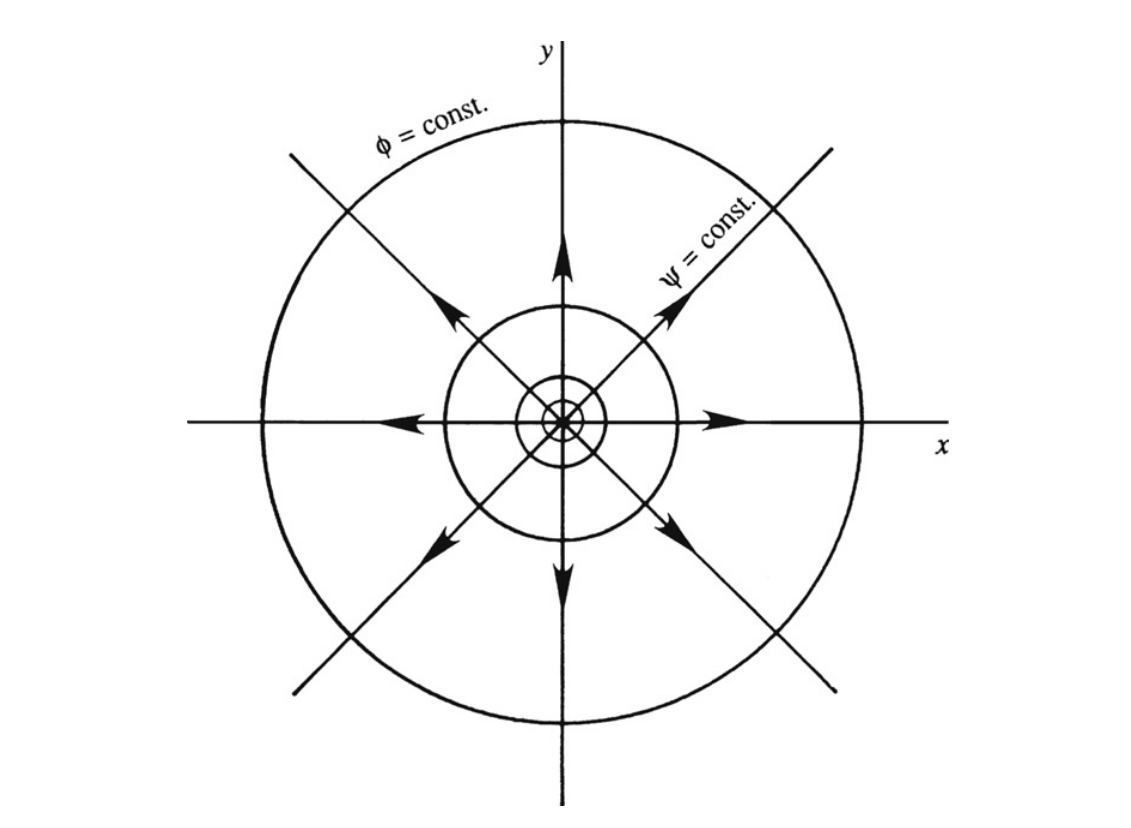
\includegraphics[width=.75\textwidth]{kcd}
	\caption{The flow field of an ideal source located at the origin of coordinates in two dimensions. The streamlines are radials and the potential lines are circles. Figure 6.5 from the KCD book}
\end{figure}

\begin{description}
	\item[(a)]
	Determine the velocity components $v_x$ and $v_y$.
	\item[(b)]
	Determine the stream function $\Psi(x,y)$.
	\item[(c)]
	Visualize the streamlines by plotting the contour lines on the stream function. Compare your results with the figure above.
	\item[(d)]
	What is the fluid mass flowing through a circle with radius $R$? What is the interpretation of the parameter $m$?
\end{description}


\section*{Exercise 3.3}
The velocity potential
\begin{align}
\Phi(x,y) &= v_\infty x + \frac{m}{2\pi}\ln\sqrt{x^2+y^2}\\
&= v_\infty r\cos\phi+\frac{m}{2\pi}\ln r
\end{align}
describes a potential flow around a half-body; see the figure below.
\begin{figure}[h!]
	\centering
	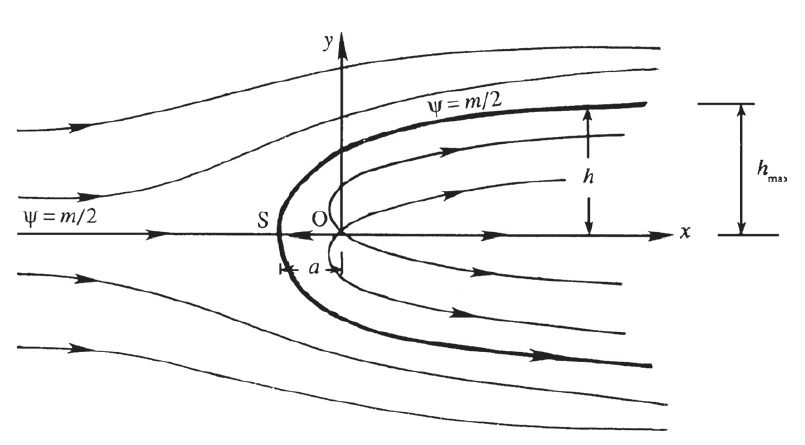
\includegraphics[width=.7\textwidth]{kcd2}
	\caption{Ideal flow past a two-dimensional half-body formed from a horizontal free stream and a point source at the origin. The boundary streamline, shown as a darker curve, is given by $\Psi=m/2$. Figure 6.7 from the KCD book}
\end{figure}

\begin{description}
	\item[(a)]
	Determine the velocity components $v_x$ and $v_y$.
	\item[(b)]
	Determine the stream function $\Psi(x,y)$.
	\item[(c)]
	Visualize the streamlines by plotting the contour lines of the stream function. Compare your results with the figure above.
\end{description}

\end{document}